\documentclass[a4paper]{article}

\usepackage[utf8]{inputenc}
\usepackage[T1]{fontenc}
\usepackage{textcomp}
\usepackage[italian]{babel}
\usepackage{amsmath, amssymb}
\usepackage{siunitx}
\usepackage{caption}
\usepackage{graphicx}
\usepackage{subcaption}
\usepackage{booktabs} % Opzionale, per tabelle più belle se vuoi (\toprule, \midrule, \bottomrule)
\usepackage{ragged2e} % Per \Centering nelle minipage
\usepackage{float} % Per [htbp]
\usepackage{fullwidth}
%\usepackage{darkmode} % Disabilitato come nell'originale
%\enabledarkmode
\usepackage[margin=2cm]{geometry}

% ======================================================
% Impostazioni siunitx (opzionale, ma utile)
% ======================================================
\sisetup{
    output-decimal-marker = {,}, % Usa la virgola come separatore decimale
    uncertainty-mode = separate, % Mostra incertezza come ±
    separate-uncertainty = true, % Forza la separazione
    locale = IT, % Impostazioni locali italiane (es. per la virgola)
    group-digits = false, % Evita di raggruppare le cifre (es. 10000 vs 10 000)
    per-mode=symbol % usa / per le unità composte es. km/h
}

% ======================================================
% Appendice con le tabelle dati
% ======================================================
\usepackage{titling}
\usepackage{appendix}
\usepackage[colorlinks=true, linkcolor=blue, citecolor=blue, urlcolor=blue]{hyperref} % Per riferimenti cliccabili (opzionale ma utile)
\usepackage[italian,nameinlink]{cleveref} % Per riferimenti più intelligenti (\cref, \Cref)

\renewcommand{\appendixname}{Appendice} % Traduce "Appendix" in "Appendice"
\renewcommand{\appendixtocname}{Appendici} % Traduce "Appendices" nel ToC
\renewcommand{\appendixpagename}{Appendici} % Traduce "Appendices" nell'header/footer

% Configurazioni cleveref per l'italiano
\crefname{section}{sezione}{sezioni}
\Crefname{section}{Sezione}{Sezioni}
\crefname{table}{tabella}{tabelle}
\Crefname{table}{Tabella}{Tabelle}
\crefname{figure}{figura}{figure}
\Crefname{figure}{Figura}{Figure}
\crefname{equation}{equazione}{equazioni}
\Crefname{equation}{Equazione}{Equazioni}
\crefname{footnote}{nota}{note}
\Crefname{footnote}{Nota}{Note}


\title{Interferometro}
\author{Alessio Ramirez, Michele Rota, Sofia Zocchi}
\date{Giugno 2025}


\begin{document}
\maketitle
\tableofcontents
\newpage

\section{Interferometro di Fabry-Perot}
\subsection{Obiettivo}
Verificare la legge che descrive la posizione dei massimi di interferenza per la configurazione di Fabry-Perot.

\subsection{Metodo}
Nella configurazione di Fabry-Perot, il laser emesso, che passa per una lente divergente, viene parzialmente riflesso nella cavità formata da due specchi paralleli e conseguentemente si hanno cammini ottici differenti per i raggi riflessi e trasmessi. 

L'interferometro di Fabry-Perot è costituito da due superfici riflettenti parallele separate da una distanza $d$ regolabile. Il fascio laser incidente viene parzialmente riflesso e trasmesso ogni volta che incontra una parete della cavità, generando multiple riflessioni all'interno di quest'ultima. I raggi che emergono dalla cavità interferiscono tra loro, producendo una figura di interferenza.

La condizione per l'interferenza costruttiva è data dalla relazione:
\begin{align}
    2d \cos \theta = N\lambda
\end{align}
dove $d$ è la distanza tra gli specchi, $\theta$ è l'angolo di incidenza rispetto alla normale, $N$ è un intero che indica l'ordine del massimo e $\lambda$ è la lunghezza d'onda della luce.

Per verificare questa legge, sono stati misurati i diametri dei massimi di interferenza proiettati sulla parete, per diversi ordini di massimi, ed è stata misurata la distanza $L$ tra la lente e la parete. Con queste misure si è ricavato l'angolo $\theta$ con la seguente relazione:
\[\theta = \arctan \left(\frac{\text{diametro}}{2L}\right)\]

\subsection{Dati}
La distanza tra lente e parete, rimasta fissa per tutte le misure, è stata misurata come $L=\SI{128 \pm 0.5}{\centi\meter}$. I dati per i vari diametri e i relativi coseni sono riportati in \cref{tab:fabry-perot-dati}.

\begin{table}[htbp]
\centering
\caption{Dati Figura di Interferenza (Fabry-Perot)}
\begin{tabular}{|c|c|c|}
\hline
Diametro & $\cos(\theta)$ & $N$ \\\hline\hline
\SI{20 \pm 1}{\milli\meter} & \SI{999.969 \pm 0.003e-3}{} & 5 \\
\SI{36 \pm 1}{\milli\meter} & \SI{999.901 \pm 0.006e-3}{} & 4 \\
\SI{48 \pm 1}{\milli\meter} & \SI{999.824 \pm 0.007e-3}{} & 3 \\
\SI{57 \pm 1}{\milli\meter} & \SI{999.752 \pm 0.009e-3}{} & 2 \\
\SI{65 \pm 1}{\milli\meter} & \SI{999.68 \pm 0.01e-3}{} & 1 \\
\hline
\end{tabular}
\label{tab:fabry-perot-dati}
\end{table}

\subsection{Analisi Dati}
È stata dunque fatta la seguente interpolazione:
\[\cos \theta = \frac{N\lambda}{2d} + A\]
con $d$ e $A$ parametri liberi e $\lambda=\SI{632.8e-9}{\meter}$ lunghezza d'onda del laser He-Ne assunta senza errore. La presenza del termine di shift $A$ è giustificata dal fatto che non è possibile determinare con certezza l'ordine assoluto $N$, con conseguenti effetti sistematici.
Il grafico dell'interpolazione è visibile in \cref{fig:fabry-perot-interpolazione}, i risultati in \cref{tab:fabry-perot-risultati}.

\begin{figure}[htbp]
\centering
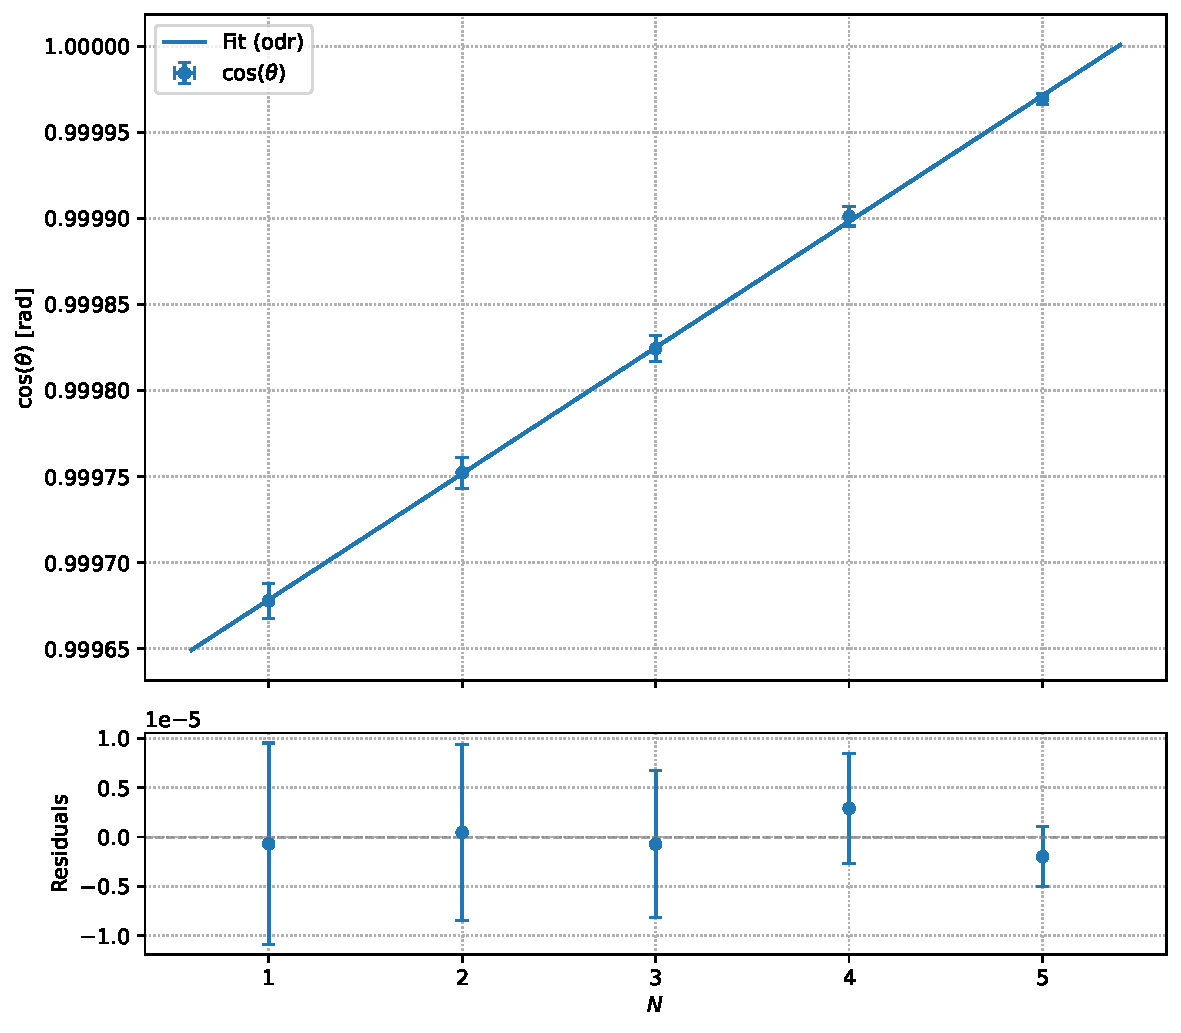
\includegraphics[width=1.0\textwidth]{./grafici/fabry_perot_interferenza.pdf}
\caption{Interpolazione della legge di Fabry-Perot}
\label{fig:fabry-perot-interpolazione}
\end{figure}

\begin{table}[htbp]
\centering
\begin{tabular}{|l|ccccc|}
\hline
parametri & A & d & $\chi^2$ & DoF & $\chi^2/\nu$ \\\hline\hline
risultati & \SI{996.0 \pm 0.077e-3}{} & \SI{4.3 \pm 1.4}{\milli\meter} & \num{2.53e-3} & 3 & \num{8.42e-4} \\\hline
\end{tabular}
\caption{Risultati Interpolazione (Fabry-Perot)}
\label{tab:fabry-perot-risultati}
\end{table}

\subsection{Conclusioni}
Dall'interpolazione si evince che la legge prevista è compatibile con l'osservazione sperimentale. L'esperimento dimostra quindi che la condizione $2d \cos \theta = N\lambda$ descrive accuratamente la posizione angolare dei massimi di interferenza nell'interferometro di Fabry-Perot.

\section{Calibrazione micrometro con interferometro di Fabry-Perot}
\subsection{Obiettivo}
Verificare la calibrazione del nonio presente nella strumentazione attraverso lo studio della figura di interferenza prodotta su uno schermo e confrontare poi la precisione ottenuta sulle misure con quella garantita dal micrometro.

\subsection{Metodo}
Una volta montato e allineato l'interferometro, mantenendo la configurazione utilizzata per lo studio della figura di interferenza, abbiamo ruotato il 
nonio di una distanza fissa $d$, corrispondente all'allargamento della cavità di Fabry-Perot. Tale variazione della dimensione della cavità causa uno
scorrimento della figura di interferenza. In particolare, dalla relazione della posizione dei massimi di interferenza si può ricavare:
\begin{align}
    2 \Delta d \cos  \theta = \Delta N \lambda
\label{eq:calibrazione-micrometro-fabry-perot}
\end{align}
Fissata l'osservazione di un punto sulla figura di interferenza, $\Delta N$ indica il numero di frange di cui si è osservato il passaggio attraverso quel punto, la lunghezza d'onda è $\lambda = \SI{632.8}{\nano\meter}$ (come indicato sul manuale PASCO) e $\theta$ rappresenta la posizione angolare a cui si trova il punto osservato, ossia l'angolo rispetto all'orizzontale di cui è inclinato il fascio.
Abbiamo variato le dimensioni della cavità 7 volte dello stesso tratto $d$ e per ciascuna di esse abbiamo misurato $\Delta N$, ricavando così 7 diversi valori di $\Delta d$, calcolato invertendo la \cref{eq:calibrazione-micrometro-fabry-perot} come:
\begin{align}
    \Delta d = \frac{\lambda \Delta N}{2\cos{\theta}}
\label{eq:calibrazione-micrometro-fabry-perot-invertita}
\end{align}

\subsection{Dati}
In \cref{tab:micrometro-fabry-perot} sono riportati i valori di $\Delta N$, ai quali è associata una sensibilità fissa $\delta_{\Delta N}$ pari ad 1 frangia, motivata dalla possibilità di errore umano nel conteggio del numero di frange osservate.

\begin{table}[htbp]
\centering
\caption{Shift di frangia osservato (interferometro di Fabry-Perot)}
\begin{tabular}{|l|ccccccc|}
\hline
Misura & 1 & 2 & 3 & 4 & 5 & 6 & 7 \\\hline\hline
$\Delta N$ & \num{24 \pm 1} & \num{23 \pm 1} & \num{23 \pm 1} & \num{24 \pm 1} & \num{25 \pm 1} & \num{25 \pm 1} & \num{23 \pm 1} \\\hline
\end{tabular}
\label{tab:micrometro-fabry-perot}
\end{table}

\subsection{Analisi dati}
Dal momento che l'angolo $\theta$ è molto piccolo, nel ricavare $\Delta d$ è stata utilizzata l'approssimazione $\cos{\theta}\approx1$, da cui consegue:
\begin{align}
    \Delta d_{\text{approx}} = \frac{\lambda \Delta N}{2}
\label{eq:calibrazione-micrometro-fabry-perot-approssimata}
\end{align}
L'imprecisione introdotta da tale considerazione è stata valutata considerando il minimo valore di $\cos{\theta}$, ossia quello che più si discosta dall'approssimazione $\cos{\theta}\approx1$, precedentemente misurato. Per quanto mostrato in \cref{tab:fabry-perot-dati}, tale valore risulta $\cos_{\min}=\num{0.99968}$.

Abbiamo quindi sostituito $\cos_{\min}$ a 1 e osservato la variazione di $\Delta d_{\text{approx}}$ rispetto a $\Delta d$, ottenendo: $\Delta d_{\text{approx}} = \num{0.99968}\Delta d$. L'approssimazione utilizzata introduce quindi un'incertezza relativa $\frac{\Delta d- \Delta d_{\text{approx}}}{\Delta d}=\sigma_{\Delta d}=\SI{0.03}{\percent}$, da confrontare poi con l'errore sul valore di $\Delta d$.
L'errore sull'allargamento della cavità di Fabry-Perot è determinato propagando gli errori rispetto alla \cref{eq:calibrazione-micrometro-fabry-perot-approssimata}, ricavando quindi:
\begin{align}
   \sigma_{\Delta d}= \frac{\lambda \delta_{\Delta N}}{2}
\label{eq:errore-calibrazione-micrometro-fabry}
\end{align}
Quanto calcolato dalle \cref{eq:calibrazione-micrometro-fabry-perot-approssimata,eq:errore-calibrazione-micrometro-fabry} è visualizzabile in \cref{tab:distanze-calibrazione-fabry-perot}.

\begin{table}[htbp]
\centering
\caption{Distanze calibrazione micrometro (interferometro di Fabry-Perot)}
\begin{tabular}{|l|ccccccc|}
\hline
Misura & 1 & 2 & 3 & 4 & 5 & 6 & 7 \\\hline\hline
$\Delta d \SI{}{\micro\meter}$ & \SI{7.6 \pm 0.3}{} & \SI{7.3 \pm 0.3}{} & \SI{7.3 \pm 0.3}{} & \SI{7.6 \pm 0.3}{} & \SI{7.9 \pm 0.3}{} & \SI{7.9 \pm 0.3}{} & \SI{7.3 \pm 0.3}{} \\\hline
\end{tabular}
\label{tab:distanze-calibrazione-fabry-perot}
\end{table}

Come si può osservare, l'errore relativo introdotto dalla sensibilità di misura risulta molto maggiore di $\sigma_{\Delta d}$; l'approssimazione ad 1 di $\cos{\theta}$ è quindi lecita.

\subsection{Conclusione}
Per ricavare la migliore stima di $\Delta d$ e per ridurne l'incertezza abbiamo calcolato la media tra i valori presenti in \cref{tab:distanze-calibrazione-fabry-perot}, ottenendo $\Delta d_{\text{best}} = \SI{7.5 \pm 0.1}{\micro\meter}$. Possiamo quindi concludere come l'utilizzo dell'interferometro ci abbia permesso di misurare distanze con una precisione pari a \SI{0.1}{\micro\meter}, dieci volte superiore rispetto alla sensibilità del micrometro.

\section{Calibrazione micrometro con interferometro di Michelson}
\subsection{Obiettivo}
L'obiettivo di questa esperienza è la calibrazione del micrometro mediante l'utilizzo di un interferometro nella configurazione di Michelson. In particolare si vuole dimostrare che la sensibilità del micrometro è inferiore alla precisione ricavata mediante l'utilizzo delle formule riguardanti l'interferenza, ovvero che la misura indiretta dello spostamento dello specchio mediante il conteggio delle frange è più precisa della misura diretta.

\subsection{Metodo}
Per effettuare le misure è stato creato un interferometro di Michelson la cui rappresentazione schematica è riportata in \cref{fig:configurazione-michelson}:

\begin{figure}[htbp]
\centering
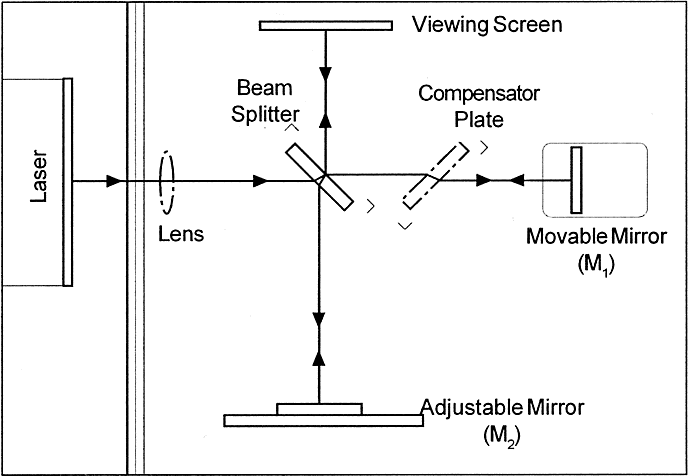
\includegraphics[width=0.9\textwidth]{grafici/configurazione michaelson.png}
\caption{Configurazione interferometro Michelson}
\label{fig:configurazione-michelson}
\end{figure}

L'interferometro è composto da un laser che invia un raggio luminoso ad una lente divergente, la quale rende i raggi della sorgente paralleli fra di loro. Il raggio collimato incide poi su uno specchio semiriflettente creando così due diversi fasci che compiono percorsi separati per poi incontrarsi nuovamente su uno schermo. I diversi raggi incidenti hanno cammino ottico diverso proprio a causa delle diverse distanze che percorrono; quando incidono sullo schermo creano dunque una figura di interferenza. Tale figura è osservabile a occhio nudo e si presenta come un'alternanza di cerchi concentrici, ciascuno relativo ad un punto di interferenza costruttiva. Variando la posizione dello specchio movibile è possibile cambiare anche il cammino ottico e dunque la figura di interferenza; in tal caso si osserverà un'alternanza di frange concentriche il cui numero varierà secondo la relazione: 
\begin{align}
    2d=\Delta N \lambda
\end{align}
dove $d$ è lo spostamento dello specchio, $\Delta N$ è il numero di frange che si alternano ad una data posizione e $\lambda=\SI{632.8}{\nano\meter}$ è la lunghezza d'onda del fascio incidente ed è un valore noto. Lo spostamento dello specchio mobile è possibile grazie all'apparato, il quale consente di variarne la posizione mediante un micrometro con scala graduata di precisione \SI{1}{\micro\meter}. Il conteggio dei massimi della figura di interferenza è stato effettuato manualmente, variando la posizione dello specchio movibile e contando ad occhio le frange.

\subsection{Dati}
Nella \cref{tab:micrometro-michelson} sono riportati i valori di $\Delta N$ contati in laboratorio per ciascuna delle 7 misure effettuate. Per effettuare tale misura abbiamo variato la posizione dello specchio di un valore costante tramite il micrometro sull'apparato e abbiamo contato il relativo numero di frange che si alternavano sullo schermo. L'errore sul numero di frange contate associato a ciascun valore è di $\pm1$ ed è motivato dal fatto che le frange si devono presentare in valori discreti e dal fatto che il conteggio è stato effettuato manualmente. 

\begin{table}[htbp]
\centering
\begin{tabular}{|l|ccccccc|}
\hline
Misura & 1 & 2 & 3 & 4 & 5 & 6 & 7 \\\hline\hline
$\Delta N$ & \num{23 \pm 1} & \num{25 \pm 1} & \num{26 \pm 1} & \num{23 \pm 1} & \num{26 \pm 1} & \num{24 \pm 1} & \num{24 \pm 1} \\\hline
\end{tabular}
\caption{Shift di frangia osservato (interferometro di Michelson)}
\label{tab:micrometro-michelson}
\end{table}

\subsection{Analisi dati}
A partire dai dati raccolti siamo riusciti a calcolare il valore di $d$ atteso tramite la formula: 
\begin{align}
    d=\frac{\Delta N \lambda}{2}
\end{align}
Otteniamo così vari valori di $d$ i quali sono riportati in \cref{tab:valori-d-michelson}:

\begin{table}[htbp]
\centering
\begin{tabular}{|l|ccccccc|}
\hline
Misura & 1 & 2 & 3 & 4 & 5 & 6 & 7 \\\hline\hline
$d$ \SI{}{\micro\meter} & \SI{7.3 \pm 0.3}{} & \SI{7.9 \pm 0.3}{} & \SI{8.2 \pm 0.3}{} & \SI{7.3 \pm 0.3}{} & \SI{8.2 \pm 0.3}{} & \SI{7.6 \pm 0.3}{} & \SI{7.6 \pm 0.3}{} \\\hline
\end{tabular}
\caption{Valore di d calcolato}
\label{tab:valori-d-michelson}
\end{table}

Il valore di $d$ finale è stato poi considerato come la media dei vari valori di $d$ ricavati, ottenendo così $d=\SI{7.7\pm0.1}{\micro\meter}$.
Siccome i valori degli spostamenti dello specchio movibile per gli esperimenti di Fabry-Perot e di Michelson sono uguali in quanto li abbiamo decisi così, ha senso fare un test di compatibilità tra i due valori ottenuti:
$t=\frac{|d_{\text{Michelson}}-d_{\text{Fabry-Perot}}|}{\sqrt{2\sigma^2}}=\num{1.42}$ che equivale a una probabilità entro $t$-sigma di $p=\num{0.84}$.

\subsection{Conclusioni}
Innanzitutto possiamo osservare che i valori di $\Delta d$ sono compatibili fra di loro. Inoltre, la sensibilità ottenuta mediante il calcolo di $\Delta d$ in maniera indiretta contando il numero di frange presenta una sensibilità maggiore rispetto a quella del micrometro, dunque è più affidabile.


\section{Interferenza con un righello}
\subsection{Obiettivo}
Stimare la lunghezza d'onda $\lambda$ di un laser attraverso l'analisi della figura di interferenza prodotta dall'illuminazione obliqua di un righello. 

\subsection{Metodo}
Quando un fascio laser monocromatico e coerente incide obliquamente su un righello metallico dotato di incisioni regolari, si verificano fenomeni di diffrazione ai bordi delle tacche che agiscono come un reticolo di diffrazione. La relazione che descrive la posizione dei massimi di interferenza in questa configurazione è: 
\begin{align}
    d(\cos\theta_i - \cos\theta_N) = N\lambda
\end{align}
dove $d=\SI{1}{\milli\meter}$ è il passo del reticolo, in questo caso la distanza tra le incisioni del righello, $\theta_i$ è l'angolo di incidenza del fascio laser, $\theta_N$ è l'angolo corrispondente al massimo di ordine $N$, e $\lambda$ è la lunghezza d'onda del laser, stimato come $\lambda=\SI{632.8}{\nano\meter}$ per il laser He-Ne utilizzato.

La distanza tra la parete e il punto di riflessione del laser sul righello è stato stimato come $L=\SI{124 \pm 5}{\centi\meter}$, il motivo di un incertezza così alta è dovuto al fatto che non è stato possibile individuare con precisione il punto di riflessione corrispondente al primo massimo. Il righello presentava una "striscia" di punti di diffrazione, tuttavia questa incertezza, come si vedrà dall'analisi dati, non ha un impatto significativo sul risultato finale. $\theta_i$ è stato dunque calcolato con $L$ e la distanza tra l'immagine del raggio indeflesso e di quello riflesso, $r$, con la seguente relazione:
\begin{align}   
    \theta_i = \arctan\left(\frac{r}{L}\right)
\end{align}
similmente $\theta_N$ è stato calcolato come:
\begin{align}
    \theta_N = \arctan\left(\frac{r_N}{L}\right)
\end{align}
dove $r_N$ è la distanza tra l'immagine del raggio indeflesso e di quello riflesso per il massimo di ordine $N$.
\subsection{Dati}
è stato misurato $r=4.7\pm0.2$, da cui $\theta_i=0.038\pm0.002$ rad, le misure di $r_N$ per i vari massimi sono riportate in \cref{tab:interferenza-righello}, insieme agli altri dati.

\begin{table}[htbp]
\centering
\begin{tabular}{|l|ccccc|}
\hline
Label & 1 & 2 & 3 & 4 & 5 \\\hline\hline
$r_N$ & 70 ± 2 mm & 85 ± 2 mm & 96 ± 2 mm & 110 ± 2 mm & 120 ± 2 mm \\\hline
$\cos(\theta_i) - \cos(\theta_N)$ & 872 ± 200 µ & 1.6 ± 0.2 m & 2.3 ± 0.3 m & 3.2 ± 0.4 m & 3.9 ± 0.4 m \\\hline
$N$ & 1 & 2 & 3 & 4 & 5 \\\hline
\end{tabular}
\caption{Dati della figura di interferenza (righello)}
\label{tab:interferenza-righello}
\end{table}

\subsection{Analisi dati}
L'interpolazione
\begin{align}
    (\cos\theta_i - \cos\theta_N) = \frac{N\lambda}{d}
\end{align}
è riportata in \cref{fig:interferenza-righello-interpolazione}, i risultati sono riportati in \cref{tab:interferenza-righello-risultati}.
\begin{figure}[htbp]
\centering
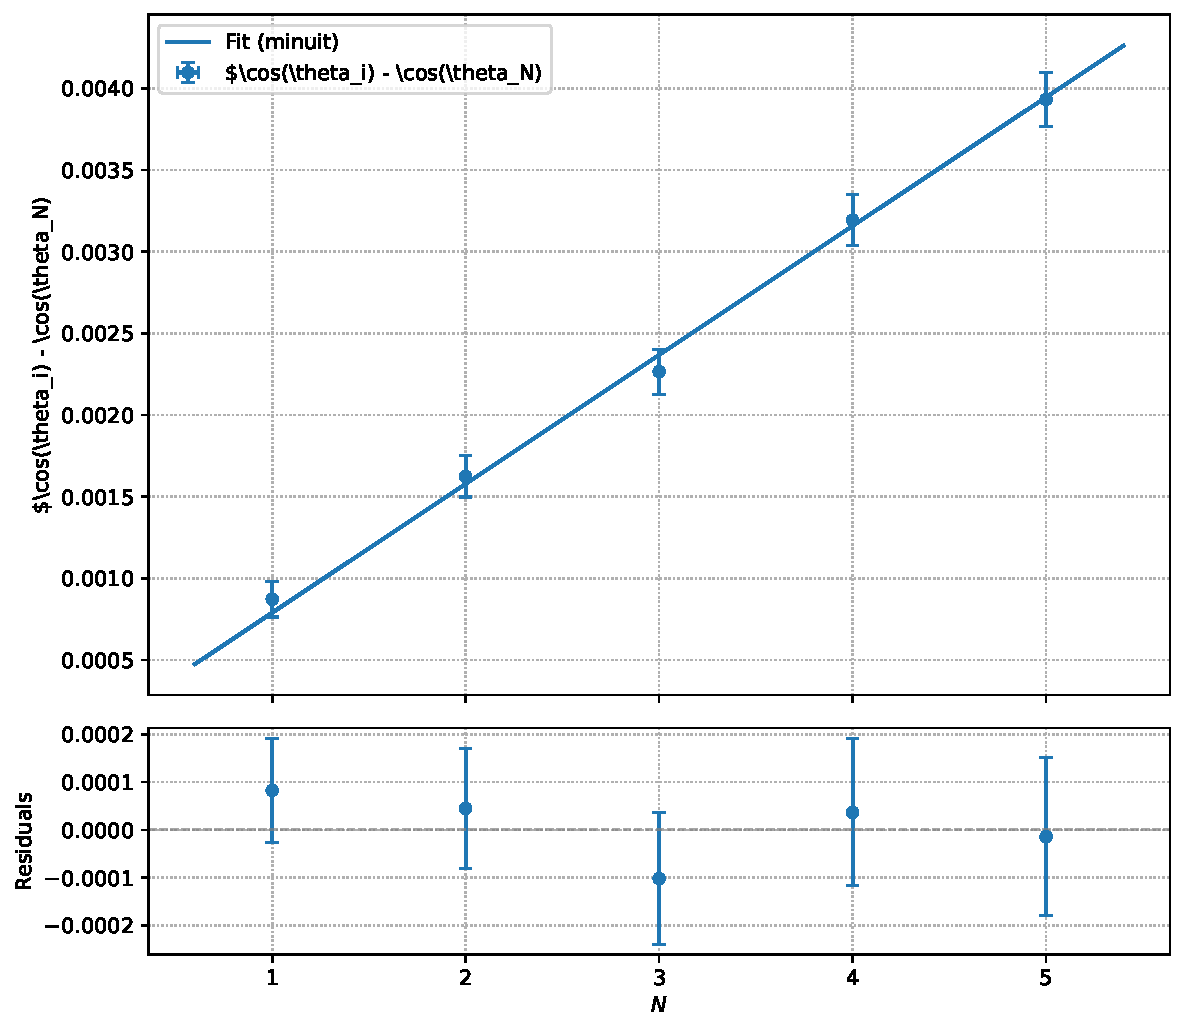
\includegraphics[width=1.0\textwidth]{./grafici/righello.pdf}
\caption{Interpolazione della legge di interferenza (righello)}
\label{fig:interferenza-righello-interpolazione}
\end{figure}

\begin{table}[htbp]
\centering
\caption{Risultati del Fit - Interferenza del Righello}
\label{tab:interferenza-righello-risultati}
\begin{tabular}{|l|cccc|}
\hline
parametri & lambd & $\chi^2$ & DoF & $\chi^2/\nu$ \\\hline\hline
fit (minuit) & 792 ± 45 n & 0.393 & 4 & 0.0983 \\\hline
\end{tabular}
\end{table}

\subsection{Conclusioni}
La lunghezza d'onda stimata è $\lambda = \SI{792 \pm 45}{\nano\meter}$, che è incompatibile con il valore noto di $\lambda = \SI{632.8}{\nano\meter}$ per il laser He-Ne ($\approx 3.5 \sigma$, p-value = 0.0001). Il fit, avendo un chi quadro ridotto, suggerisce che la legge usata descriva correttamente il fenomeno, dal punto di vista della relazione lineare tra $\cos(\theta_i) - \cos(\theta_N)$ e $N$, e la grossa incertezza sulla misura di $L$ non compromette questo risultato, infatti ipotizzando un errore del millimetro risulterebbe comunque un chi quadro ridotto di 0.328. Ipotizziamo dunque che la legge racchiuda correttamente la fisica dietro il fenomeno, ma manchi di qualche fattore correttivo dovuto alla non idealità del sistema. 
\end{document}